\documentclass [a4paper, 12pt] {article}
\usepackage{tikz}
\usetikzlibrary{calc}

% \usepackage{titling}
% \pretitle{\begin{center}\LARGE\bfseries}
% \posttitle{\par\end{center}\vskip 0.5em}
% \preauthor{\begin{center}\large}
% \postauthor{\par\end{center}}
% \predate{\begin{center}\footnotesize}
% \postdate{\par\end{center}}

\title{Data Structure}
% \posttitle{\par\end{center}\vspace{-1.5em}\begin{center}\large Graph\end{center}}
\author{Pranto}
\date{\today}
\begin{document}

\maketitle
\section{Graph 1}
Lets make the grpah of ED task 1.
% For Line Spacing.
\vspace{20pt}

\begin{center}
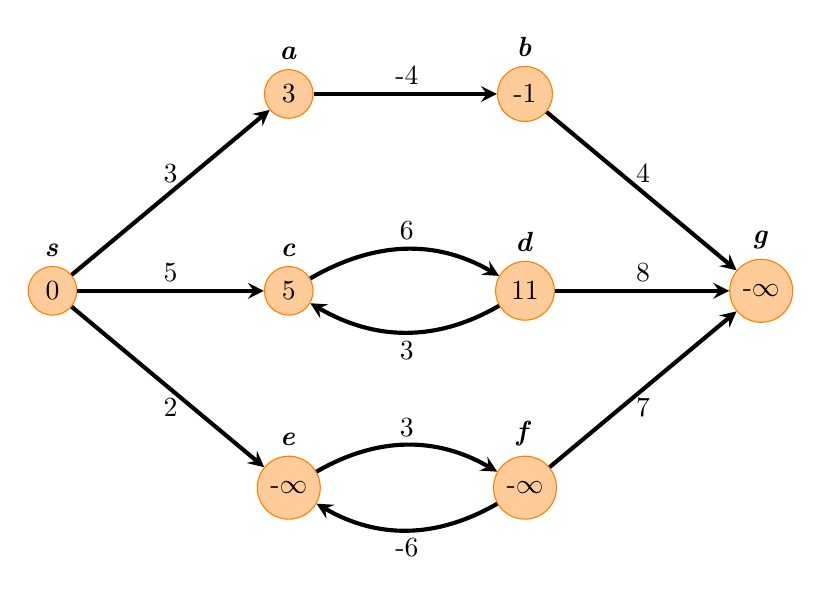
\begin{tikzpicture}[]

% Nodes
    \node[draw = orange, circle, fill = orange!40] (A) at (0, 0) {0};
    \node[draw = orange, circle, fill = orange!40] (B) at (3, 0) {5};
    \node[draw = orange, circle, fill = orange!40] (C) at (6, 0) {11};
    \node[draw = orange, circle, fill = orange!40] (D) at (9, 0) {-$\infty$};
    \node[draw = orange, circle, fill = orange!40] (E) at (3, 2.5) {3};
    \node[draw = orange, circle, fill = orange!40] (F) at (6, 2.5) {-1};
    \node[draw = orange, circle, fill = orange!40] (G) at (3, -2.5) {-$\infty$};
    \node[draw = orange, circle, fill = orange!40] (H) at (6, -2.5) {-$\infty$};

% Directions
    \draw [->, > = stealth, line width = 1.5pt] (C) -- (D);
    \draw [->, > = stealth, line width = 1.5pt] (A) -- (E); 
    \draw [->, > = stealth, line width = 1.5pt] (E) -- (F); 
    \draw [->, > = stealth, line width = 1.5pt] (F) -- (D);
    \draw [->, > = stealth, line width = 1.5pt] (A) -- (G);
    \draw [->, > = stealth, line width = 1.5pt] (A) -- (B);
    \draw [->, > = stealth, line width = 1.5pt] (H) -- (D);
    
% Bidirections
    \draw [->, > = stealth, line width = 1.5pt] (B) to [out = 30, in = 150] (C);
    \draw [->, > = stealth, line width = 1.5pt] (C) to [out = -150, in = -30] (B);
    \draw [->, > = stealth, line width = 1.5pt] (G) to [out = 30, in = 150] (H);
    \draw [->, > = stealth, line width = 1.5pt] (H) to [out = -150, in = -30] (G);

% Nodes Levels
    \node [above] at (A.north) {\textbf{\textit{s}}};
    \node [above] at (B.north) {\textbf{\textit{c}}};
    \node [above] at (C.north) {\textbf{\textit{d}}};
    \node [above] at (D.north) {\textbf{\textit{g}}};
    \node [above] at (E.north) {\textbf{\textit{a}}};
    \node [above] at (F.north) {\textbf{\textit{b}}};
    \node [above] at (G.north) {\textbf{\textit{e}}};
    \node [above] at (H.north) {\textbf{\textit{f}}};

% Edges Levels
    \node[above] at ($(A)!0.5!(B)$) {5};
    \node[above = 15pt] at ($(B)!0.5!(C)$) {6};
    \node[below = 15pt] at ($(C)!0.5!(B)$) {3};
    \node[above] at ($(C)!0.5!(D)$) {8};
    \node[above] at ($(A)!0.5!(E)$) {3};
    \node[above] at ($(E)!0.5!(F)$) {-4};
    \node[above] at ($(F)!0.5!(D)$) {4};
    \node[below] at ($(A)!0.5!(G)$) {2};
    \node[above = 15pt] at ($(G)!0.5!(H)$) {3};
    \node[below = 15pt] at ($(H)!0.5!(G)$) {-6};
    \node[below] at ($(H)!0.5!(D)$) {7};

\end{tikzpicture}  
\end{center} 
\end{document}
